\documentclass{article}

\usepackage{geometry}
\usepackage{amsmath}
\usepackage{graphicx}
\usepackage{listings}
\usepackage{hyperref}
\usepackage{multicol}
\usepackage{fancyhdr}
\pagestyle{fancy}
\hypersetup{ colorlinks=true, linkcolor=black, filecolor=magenta, urlcolor=cyan}
\geometry{ a4paper, total={170mm,257mm}, top=20mm, right=20mm, bottom=20mm, left=20mm}
\setlength{\parindent}{0pt}
\setlength{\parskip}{1em}
\renewcommand{\headrulewidth}{0pt}
\lhead{Competitive Programming - Arkavidia V}
\fancyfoot[CE,CO]{\thepage}
\lstset{
    basicstyle=\ttfamily\small,
    columns=fixed,
    extendedchars=true,
    breaklines=true,
    tabsize=2,
    prebreak=\raisebox{0ex}[0ex][0ex]{\ensuremath{\hookleftarrow}},
    frame=none,
    showtabs=false,
    showspaces=false,
    showstringspaces=false,
    prebreak={},
    keywordstyle=\color[rgb]{0.627,0.126,0.941},
    commentstyle=\color[rgb]{0.133,0.545,0.133},
    stringstyle=\color[rgb]{01,0,0},
    captionpos=t,
    escapeinside={(\%}{\%)}
}

\begin{document}

\begin{center}
    \section*{J. Jalur kereta}

    \begin{tabular}{ | c c | }
        \hline
        Batas Waktu  & 1s \\
        Batas Memori & 512MB \\
        \hline
    \end{tabular}
\end{center}

\subsection*{Deskripsi}

Negeri Ganesha memiliki peta jalur kereta yang terdiri dari $N$ jalur kereta, menghubungkan kota A dan kota B.
Peta jalur kereta ini sangat rumit, sehingga peta jalur kereta ini hanya boleh dilewati oleh kereta dari kota A ke B, tidak sebaliknya.

\begin{multicols}{2}
\begin{center}
    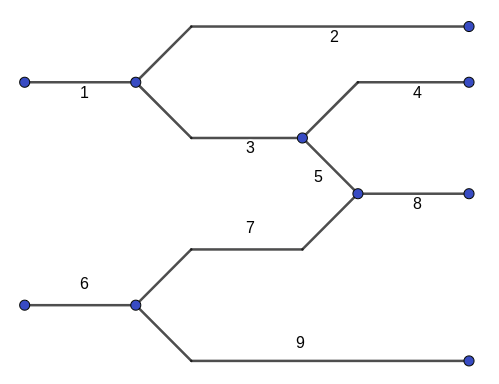
\includegraphics[width=200px]{sample-1}
\end{center}

Di samping ini merupakan contoh peta jalur kereta yang terdiri dari 8 jalur kereta (kiri adalah kota A dan kanan adalah kota B).
Hanya terdapat 2 jenis persimpangan, yakni:
\begin{enumerate}
    \setlength{\itemsep}{0pt}
    \item Sebuah jalur terbagi menjadi dua jalur berbeda
    \item Dua jalur berbeda bergabung menjadi satu jalur
\end{enumerate}
Sebagai contoh, persimpangan 1, 2, 3 merupakan persimpangan jenis 1 dan persimpangan 3, 6, 7 merupakan persimpangan jenis 2.
\end{multicols}

Menurut Arvy, penempatan dua kereta di jalur $x$ dan $y$ dianggap bagus jika $x$ tidak bisa dicapai dari $y$ dan $y$ tidak bisa dicapai dari $x$ (ingat kalau semua rel hanya satu arah, dari kiri ke kanan).
Kini ia bertanya, berapa maksimum kereta yang bisa ditempatkan sehingga penempatan setiap dua pasang kereta dianggap bagus oleh Arvy.

\subsection*{Format Masukan}
Baris pertama terdiri dari satu bilangan bulat positif $T$ ($1 \leq T \leq 10$), menyatakan banyaknya kasus uji.
Tiap kasus uji diawali dengan bilangan $N$ dan $M$ ($1 \leq N, M \leq 10.000$) menyatakan banyaknya persimpangan dan banyaknya jalur.
$N$ baris berikutnya terdiri dari 4 bilangan dengan format:
\begin{itemize}
    \setlength{\itemsep}{0pt}
    \item \lstinline{1 a b c}, menandakan adanya persimpangan tipe 1, yakni jalur nomor a bercabang menjadi b dan c.
    \item \lstinline{2 a b c}, menandakan adanya persimpangan tipe 2, yakni jalur nomor a dan b bergabung menjadi c.
\end{itemize}

\subsection*{Format Keluaran}
Tuliskan $T$ baris, masing-masing berisikan banyaknya kereta maksimum yang dapat ditempatkan sehingga penempatan tiap dua pasang kereta dianggap bagus oleh Arvy.

\pagebreak

\begin{multicols}{2}
\subsection*{Contoh Masukan}
\begin{lstlisting}
1
4 9
1 1 2 3
1 3 4 5
1 6 7 9
2 5 7 8
\end{lstlisting}
\columnbreak
\subsection*{Contoh Keluaran}
\begin{lstlisting}
4
\end{lstlisting}
\vfill
\null
\end{multicols}

\subsection*{Penjelasan}
Pada kasus uji pertama, peta jalur kereta dapat digambarkan seperti peta yang ada di deskripsi soal. Penempatan yang maksimum salah satunya dengan menempatkan kereta pada nomor $2, 3, 7, 9$.

\end{document}